\section{Aufbau und Durchführung}
\label{sec:aufbau}
\FloatBarrier

	Alle verwendeten Geräte und deren Aufbau sind in Abbildung \ref{fig:aufbau} zu sehen.
	Nach dem Positionieren der Quelle im Quellenhalter empfängt der aktive Detektor die $\gamma$-Quanten und sendet ein entsprechendes Signal an den Vielkanalanalysator.
	Dieser erhöht nun je nach Energie des Eingabeimpulses die Counts eines entsprechenden Kanals.
	Wird statt einem HP-Ge-Detektor ein Szintillationsdetektor verwendet, so wird vor dem Vielkanalanalysator noch ein Photoelektronenvervielfacher oder auch Photomultiplier benötigt, der die empfangenen Signale des Detektors verstärkt.

	\begin{figure}[htb]
		\begin{subfigure}[b]{0.5\textwidth}
			\centering
			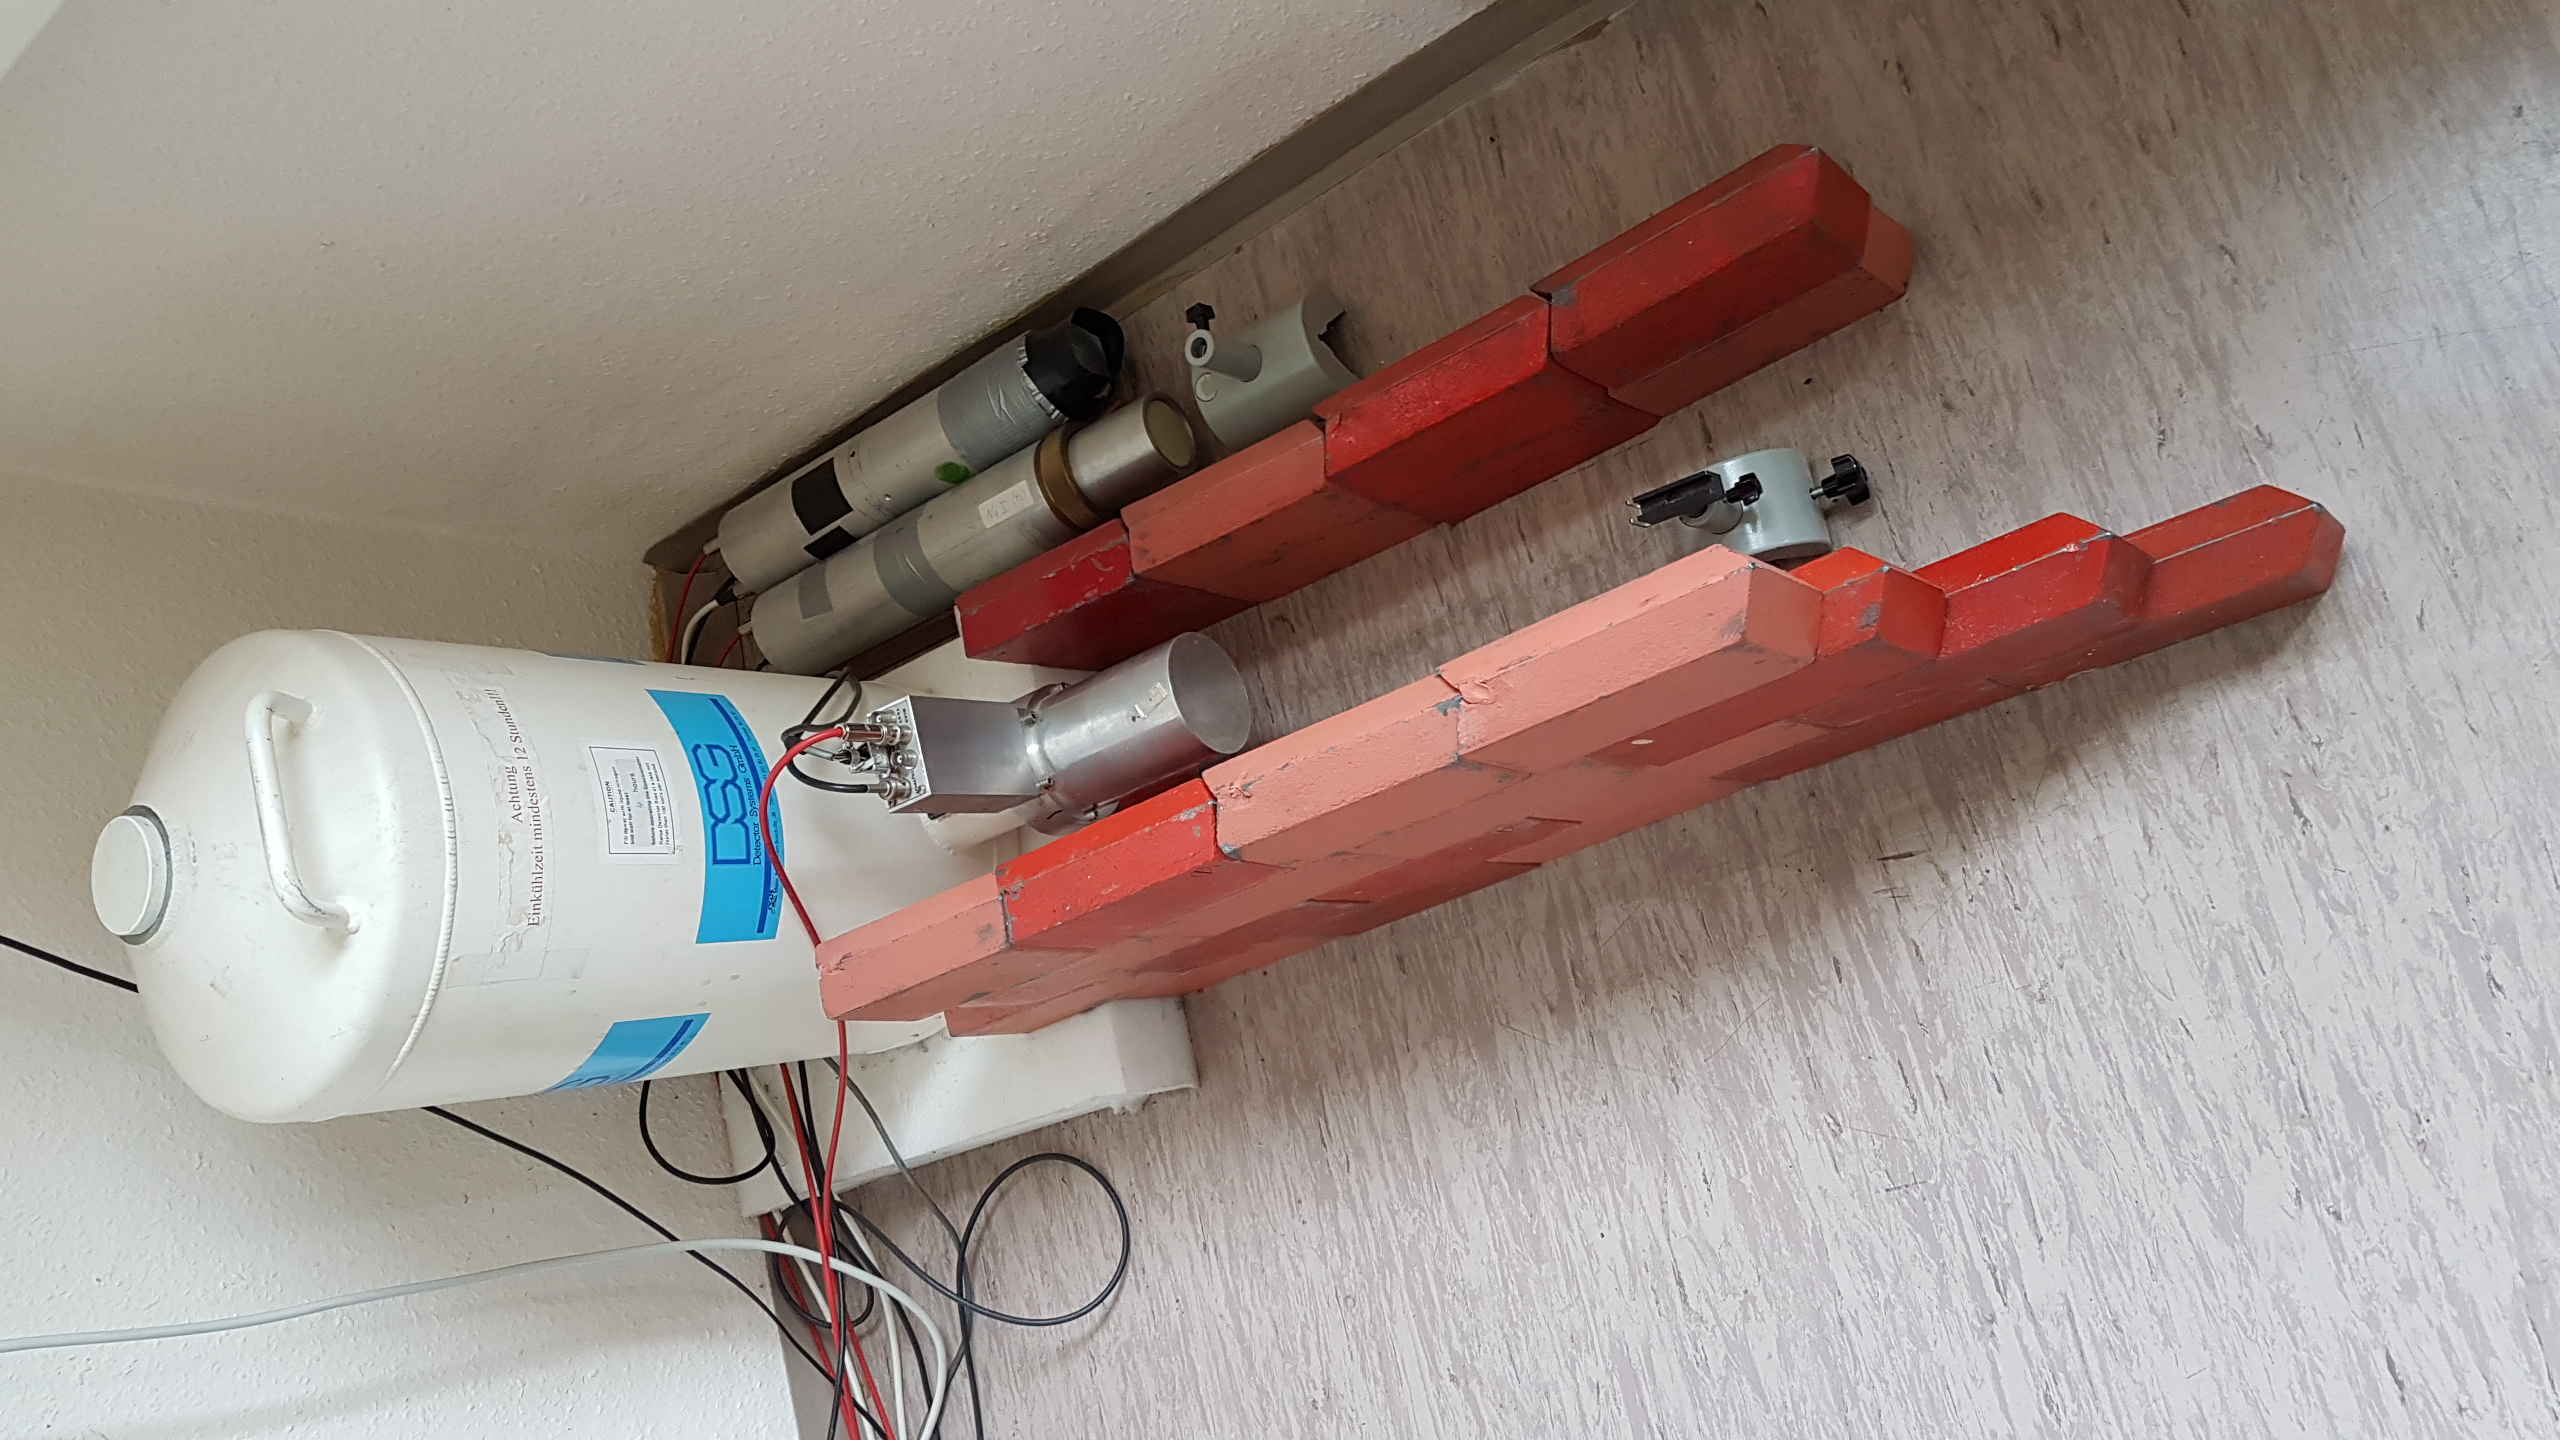
\includegraphics[scale=0.1, angle=-90]{pic/20160613_152508.jpg}
			\caption{Detektoren und Quellenhalter}
		\end{subfigure}
		\begin{subfigure}[b]{0.5\textwidth}
			\centering
			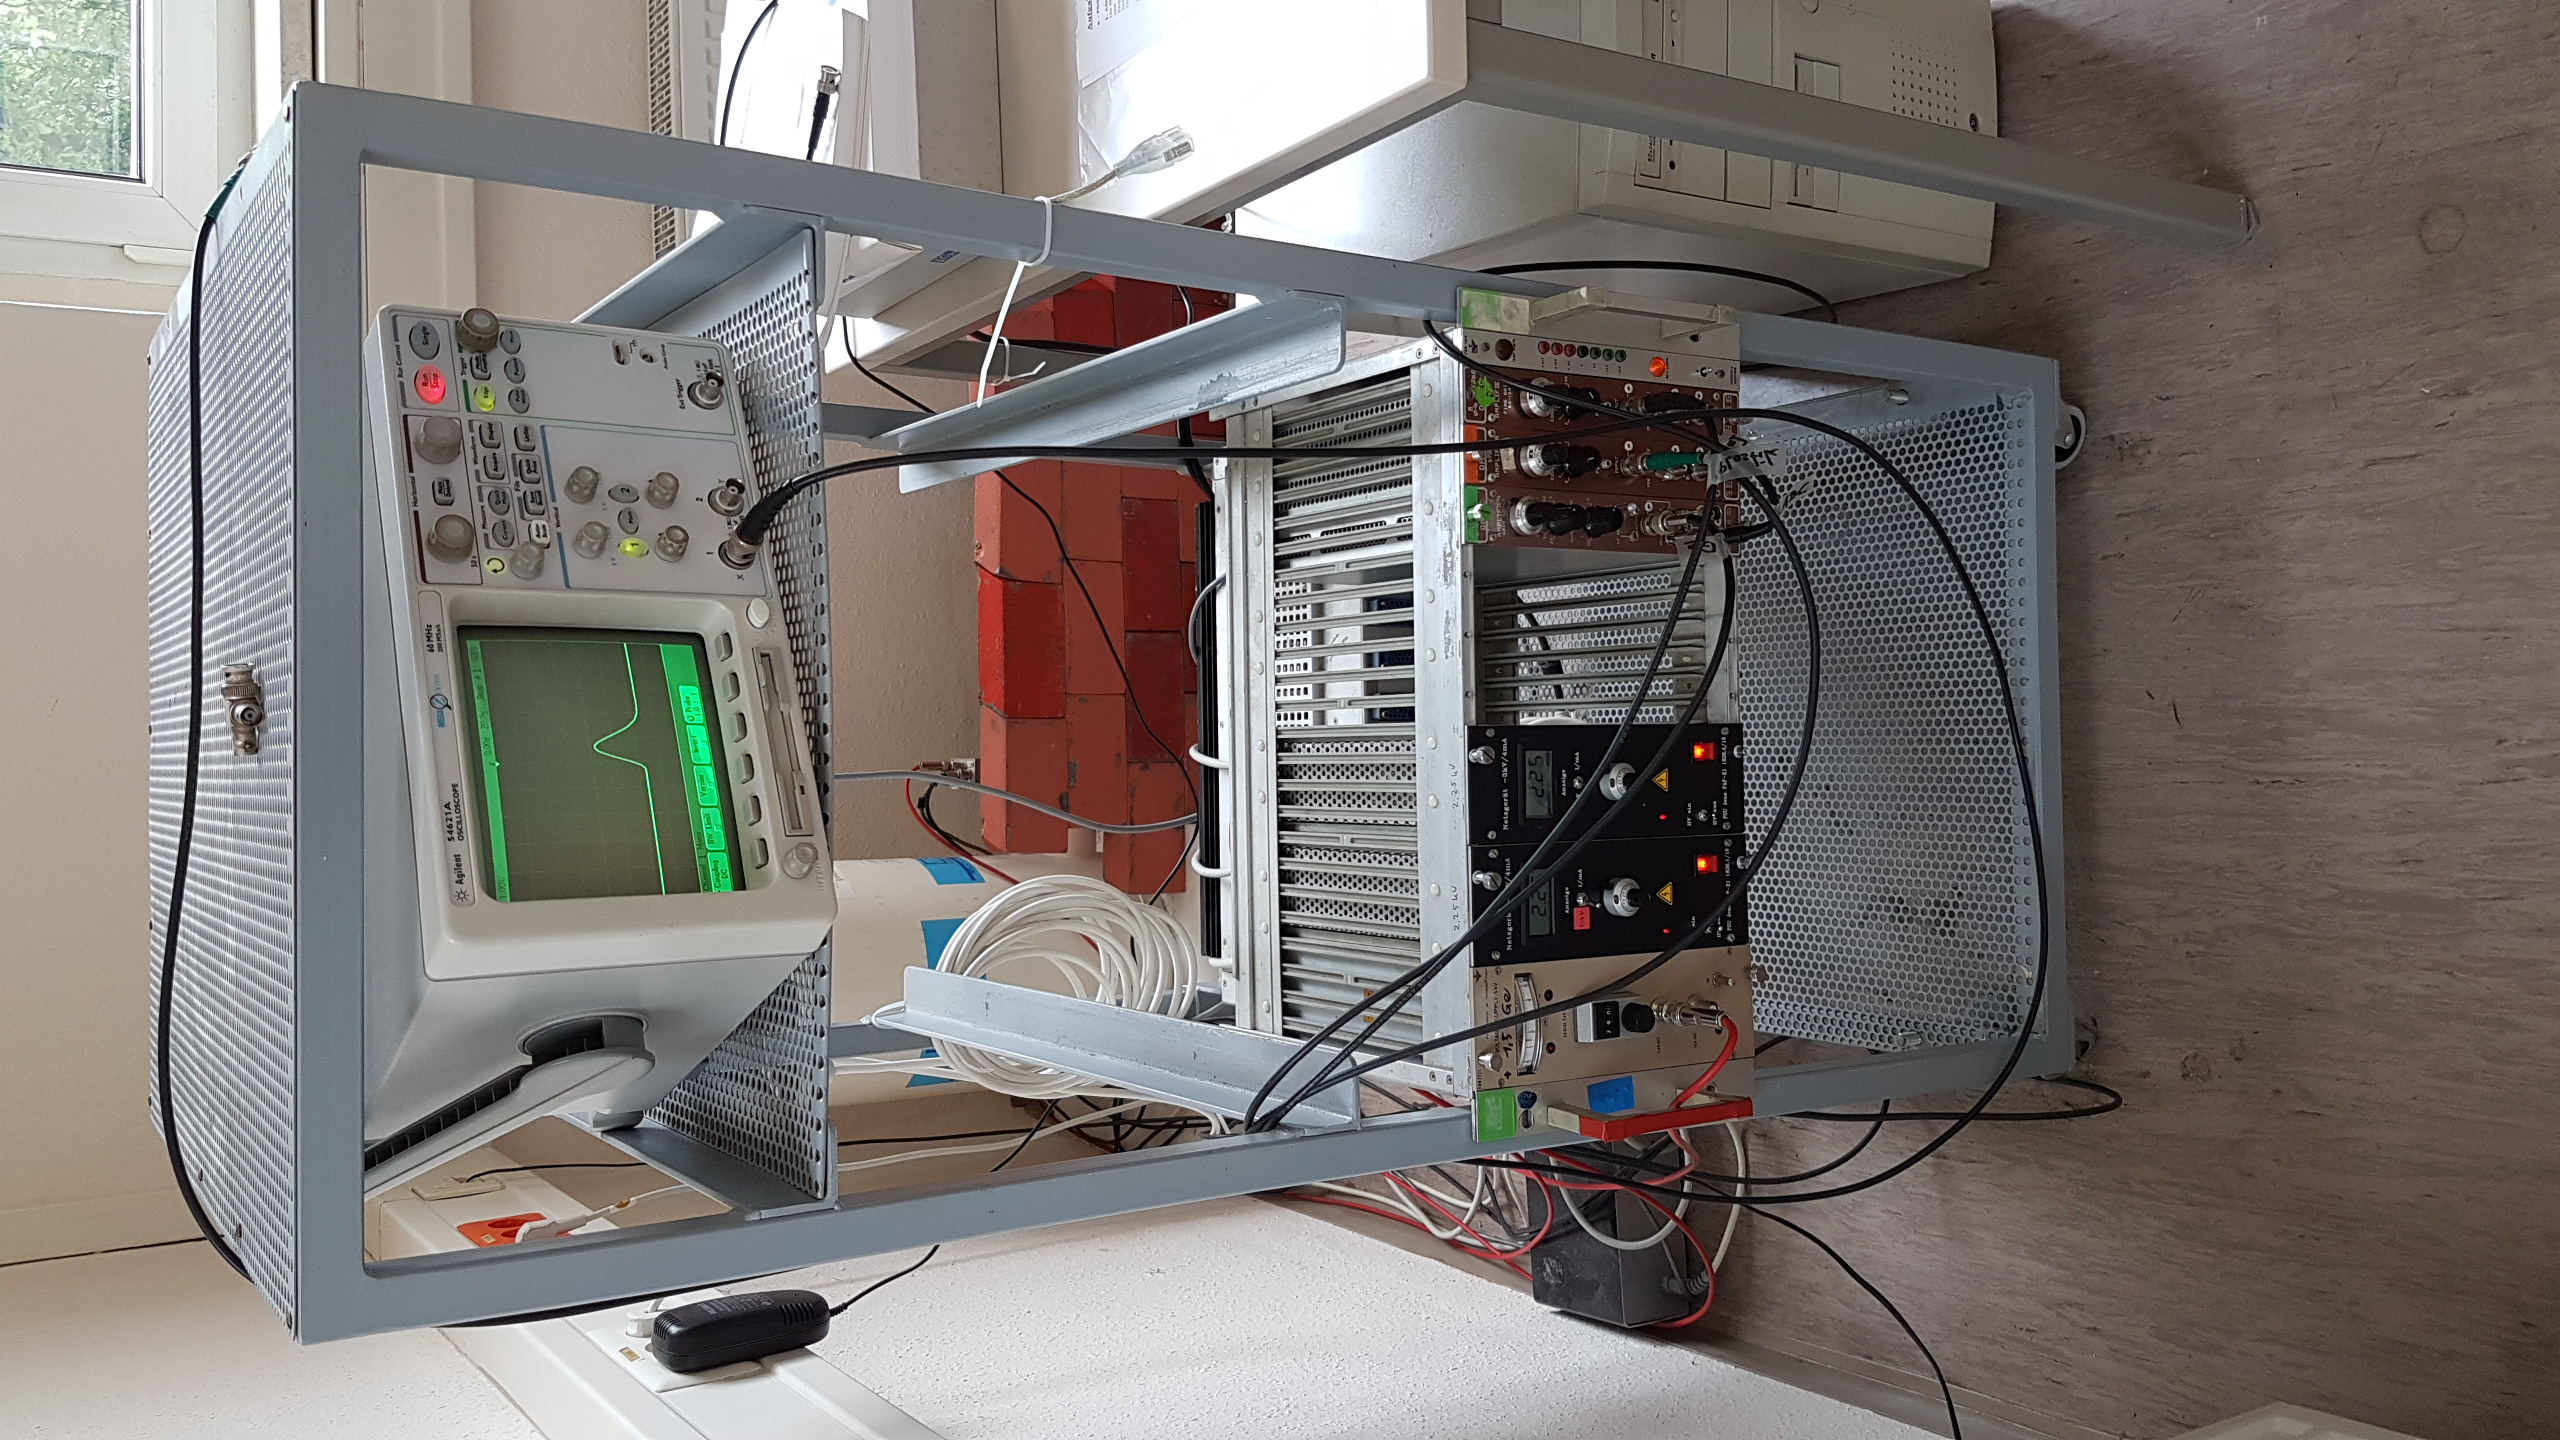
\includegraphics[scale=0.1, angle=-90]{pic/20160613_152531.jpg}
			\caption{elektronische Geräte}
		\end{subfigure}
		\caption{verwendete Geräte und deren Aufbau}
		\label{fig:aufbau}
	\end{figure}

	Nachdem der Vielkanalanalysator das Signal empfangen und in einen Kanal eingeteilt hat, wird die Information an einen Computer gesendet, der die gemessenen Counts über deren Kanäle darstellt.
	Dieser ermöglicht es dann die Daten zu speichern, sodass sie später für die Auswertung verfügbar sind.

	Die zu analysierenden Quellen wurden außerhalb der Messungen in Bleibehältern, welche in Abbildung \ref{fig:proben} zu sehen sind, aufbewahrt.

	\begin{figure}[htb]
		\centering
		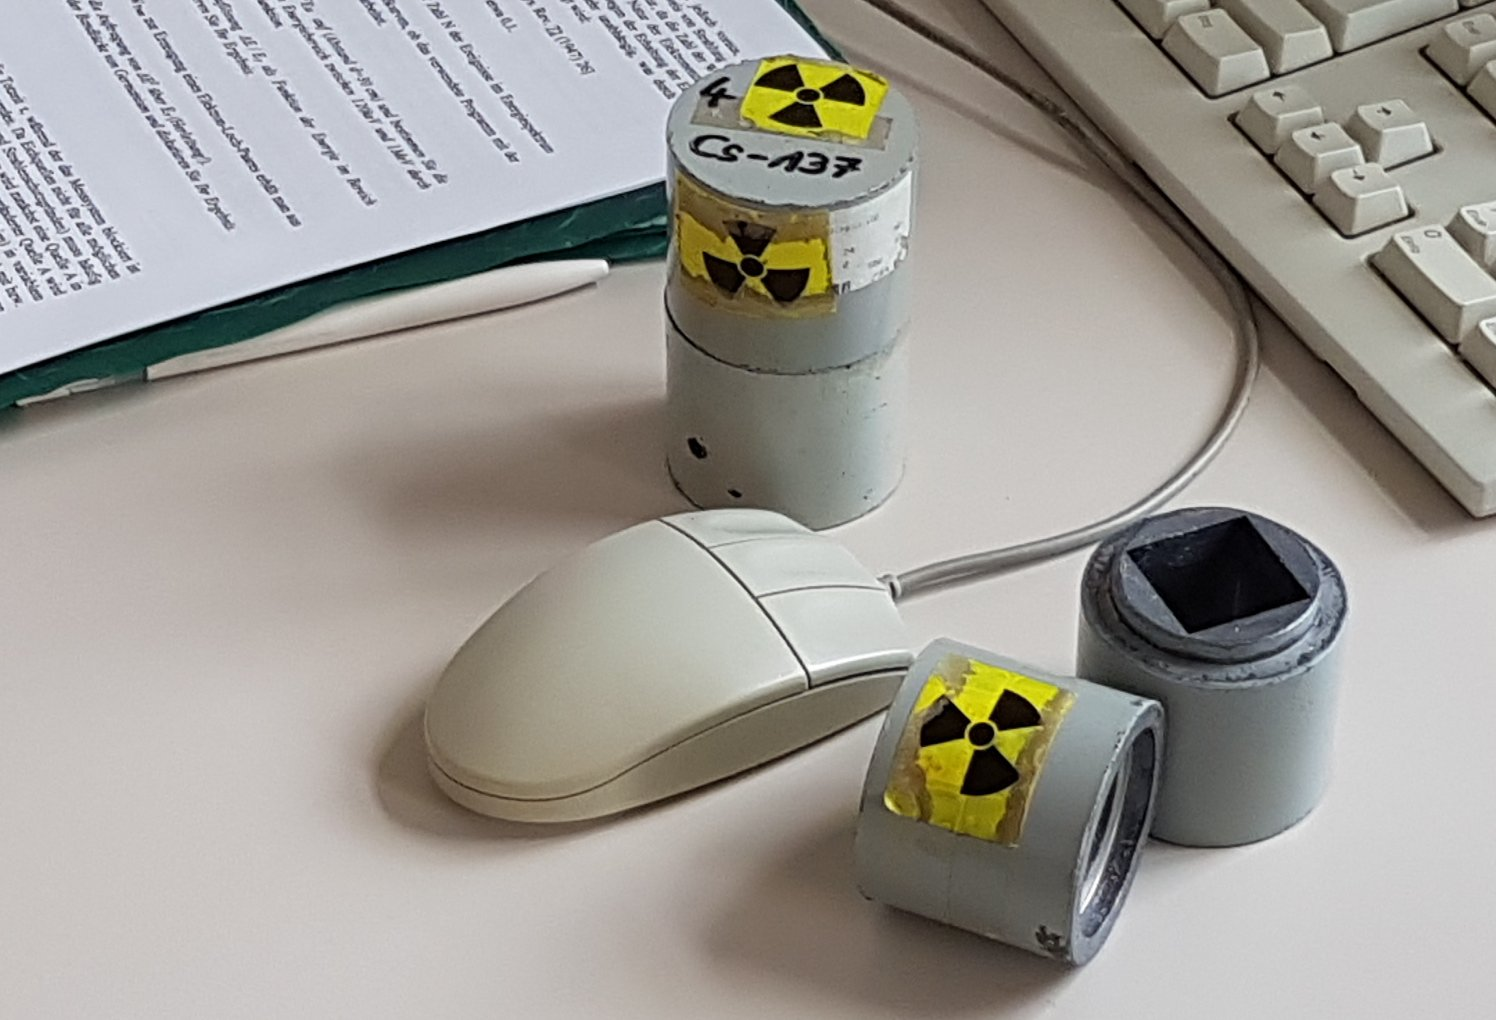
\includegraphics[scale=0.2]{pic/proben.jpg}
		\caption{Bleibehälter für Proben}
		\label{fig:proben}
	\end{figure}

% section aufbau
